\documentclass{article}

\usepackage{graphicx}
\usepackage{subfig}
\usepackage{amsmath}

\usepackage{listings}

\newcommand{\norm}[1]{\| #1 \|}

\title{Three-dimensional Turbulent Channel}

\date{}

\begin{document}

\maketitle

\section{Introduction}
This case provides a description for three-dimensional turbulent channel 
($Re_\tau = 1000$) that is run using a wall-modeled large-eddy simulation (WMLES) paradigm.
A constant body force is applied to the domain that drives the flow. The objective 
of this laboratory case is to understand the one-dimensional exchange-based
wall-modeling approach that is common in the WMLES literature, see~\cite{larsson2016}.
Full production runs would require increased mesh resolution - an exercise left to the
reader.

\section{Domain}
The three-dimensional geometry for this tutorial is captured in Figure~\ref{fig:geom}. 
The top and bottom boundaries are no-slip, while all others are periodic (both spanwise
and streamwise). The domain length (streamwise direction, x), width (spanwise direction, z) and
height (vertical direction, y) are $2\pi$ \!x $2/3\pi$ \!x $2$, respectively.

\begin{figure}[!htbp]
  \centering
  {
   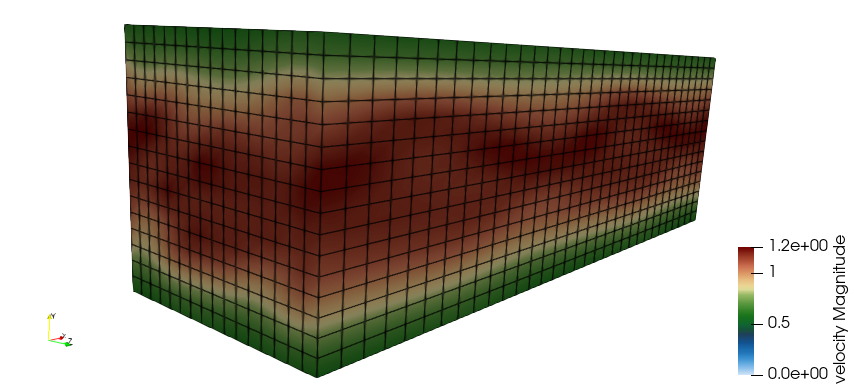
\includegraphics[height=1.25in]{images/3d_hex8_turb_channel_geom.png}
  }
  \caption{Three-dimensional channel flow.}
  \label{fig:geom}
\end{figure}

\section{Theory}
General details on the WMLES technique can be found in~\cite{larsson2016}, however, in short
this is a modeling approach to alleviate the substantial mesh resolution requirement that is
required to adequately resolve turbulent boundary layers. For a classic description of 
mesh requirement scaling, the reader is referred to~\cite{chapman}. For the 
target $Re_\tau = 1000$ configuration, which is based on the channel half-height, the density ($\rho$) 
and viscosity ($\mu$) specification are $1.0$ and $5.0 \times 10^{-5}$, respectively. The corresponding
constant body force is $2.5 \times 10^{-3}$. 

Rather than resolving the turbulent boundary layer through increased mesh resolution, which 
would be characterized as a wall-resolved LES (WRLES), the wall shear stress can be 
modeled using an equilibrium-based approach that exercises the classic law of the wall
expression,

\begin{align}
u^+ = {u_{\|} \over u_{\tau}} 
    = { 1 \over \kappa } \ln \left(y^+\right) + C.
\label{law_wall}
\end{align}
Above, $u_{\|}$ is the parallel velocity, $u_\tau$ is the wall friction velocity, $\kappa$ is a constant
(generally, 0.41), $y^+$ is the dimensionless vertical height, and $C$ is a constant that varies
based on the estimated surface roughness (generally $~$5.1). The dimensionless vertical height is defined
by,
%
\begin{align} 
        y^+ =  {{ \rho Y_p u_{\tau}} \over {\mu }},
\label{yplus}
\end{align}
where $Y_p$ is the first mesh spacing distance.

Given a parallel velocity, computational first mesh spacing distance and a set of properties (density, 
viscosity, and surface roughness), the above expression can be solved iteratively to obtain the friction 
velocity and subsequent wall shear stress, $\tau_w = \rho u^2_\tau$. The integrated wall shear stress forms
the wall boundary contribution to the momentum equation that is partitioned based on the vector components 
of the parallel, or tangential velocity component to the wall.

\section{ODE-based Exchange}
Assuming an isothermal configuration in which the viscosity and density are constant, the wall shear stress 
can be modeled using an ordinary-differential equation (ODE) approach~\cite{larsson2016} where the 
following underlying one-dimensional equation is solved:

\begin{align} 
       -\frac{d}{dy}\left[ \left(\mu + \mu^t\right) \frac{dU}{dy}  \right] = 0.0,
\label{odeExpression}
\end{align}
where,
%
\begin{align} 
       \mu^t = \kappa \rho \sqrt{\frac{\tau_w}{\rho}} y \left[1 - \exp\left(-y^*/A^+\right)\right]^2,
\label{odeExpressionMuT}
\end{align}

\begin{align} 
       y^* =  {{ \rho y u_{\tau}} \over {\mu }} =  {{ \rho y } \over {\mu}}\sqrt{\frac{\tau_w}{\rho}} 
       =  \frac{y \sqrt{\rho \tau_w}}{\mu}.
\label{odeExpressionYStar}
\end{align}

The constants $A^+$ and $\kappa$ are 17.0 and 0.41, respectively, while the distance $y$ is relative
to the wall location and proceeds to the physical exchange location, $\Delta$.

The above set of equations can be discretized over a one-dimensional coordinate system using a finite volume or 
finite element method. The system mirrors a stationary, i.e., without a time derivative,  one-dimensional 
variable-coefficient diffusion solve since 
the effective viscosity varies by height. Moreover, the solution procedure is nonlinear as the wall shear 
stress is a obtained from the iteratively-converging velocity profile, i.e., $\tau_w = \mu \frac{dU}{dy}$. 
This profile can be computed using a one-sided gradient at the wall, or $y=0$ location. 

\subsection{Solution Procedure}
A simple node-based iteration solution procedure/algorithm can be represented as follows:

\begin{enumerate}

\item Define the one-dimensional set of nodes (or points) that may include variable mesh spacing 
near the wall for increased wall shear stress calculation accuracy. Here, the wall location may be 
$y = 0$ and the final point location the exchange distance, $y = \Delta$.

\item Guess a wall shear stress, $\tau_w$ and compute the turbulent viscosity from Eq.~\ref{odeExpressionMuT}
at each point in the domain.

\item Assemble and solve a matrix system for Eq.~\ref{odeExpression} whose effective 
nodal viscosity, i.e.,  $\mu + \mu^t$, is variable as the values are a function of height
and the current wall shear stress. The integration point effective viscosity can be interpolated 
from the surrounding nodal values. The boundary conditions for velocity are simply: $U = 0$ at $y =0$, 
and $U = U^X$ at $y = \Delta$ (here, let $U^X$ be the parallel velocity at the exchange point).
For a vertex-based scheme, the rows for each known boundary condition can be modified to enforce 
the Dirichlet condition. 

\item Compute an updated wall shear stress from the recently computed velocity profiled obtained in 
step 3 above.

\item Determine the error between the previous and most current wall shear stress. If this error is 
sufficiently small, then the system has been converged. Otherwise, return to step 2 with the latest 
wall shear stress and repeat. A new matrix system must be computed at each iteration since the 
matrix coefficients are changing due to an updated effective viscosity. 

\end{enumerate}

For more information, the webpage of~\cite{larssonWebpage} can be a useful guide, especially if a 
non-isothermal system is desired to be modeled.

\subsection{Example ODE Profile}
As an example of the WMLES approach, the untransformed law of the wall dimensionless coordinate velocity profiles 
for a turbulent flow past an elevated cylinder are depicted in Figure~\ref{fig:ode}. In this figure, both the ODE- and
law of the wall, i.e., Eq.~\ref{law_wall} are shown. Various mesh points and bias factors are captured along with the 
converged wall shear stress.

\begin{figure}[!htbp]
  \centering
  {
   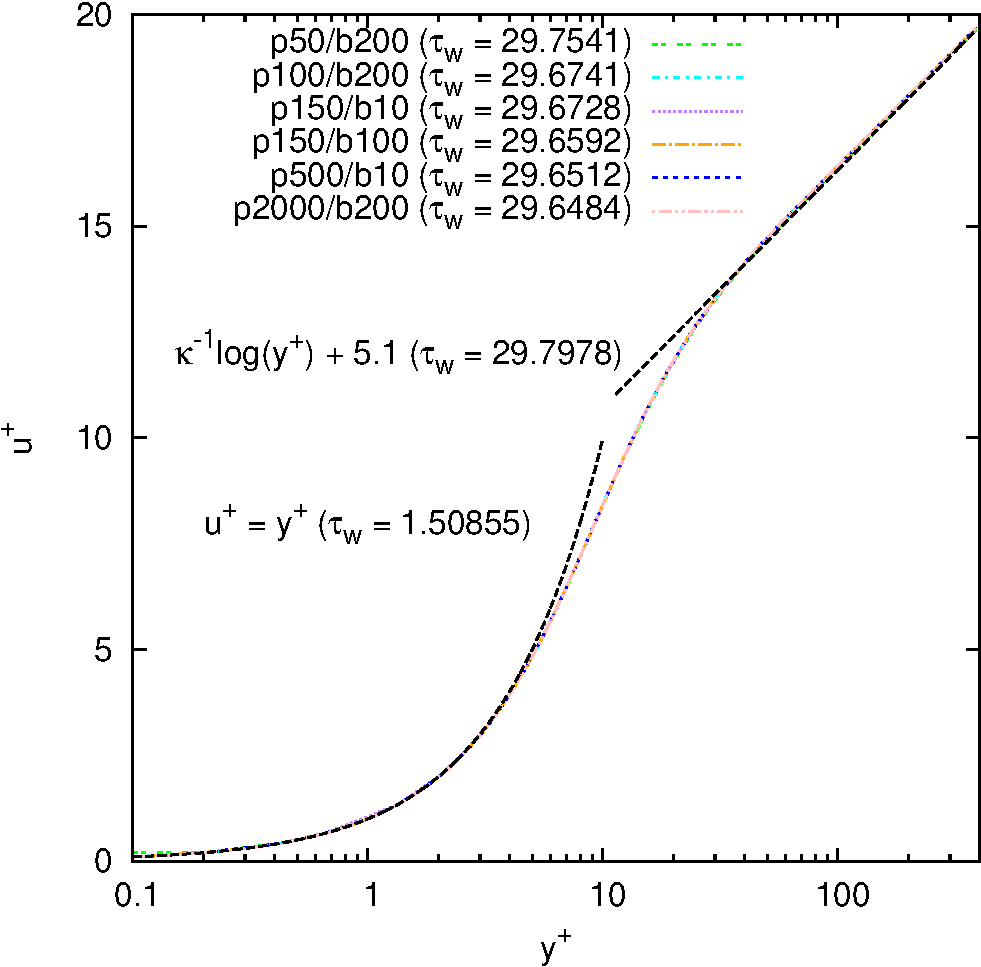
\includegraphics[height=3.0in]{images/ode_extrude-crop.pdf}
  }
  \caption{Normalized velocity and normal distance plot showcasing the ODE-based profile and compared to laminar
and standard law of the wall. In this configuration the specifications are as follows: parallel exchange velocity, 
3.39 $m/s$; density, 1000 $kg/m^3$; viscosity, $8.9 \times 10^{-4}$ $kg/m-s$; exchange location outer distance, 
0.002 $m$; constants: $A^+$ 17 and $\kappa$ 0.41. In this plot, ``p'' represents the number of points while 
``b'' represents the bias factor, or the ratio between the last and first mesh spacing.}
  \label{fig:ode}
\end{figure}

\section{Discussion Points}

There are several interesting activities associated with this sample case including
the following:

\begin{itemize}

\item Replicate Fig.~\ref{fig:ode} using the specifications provided in this figure for parallel exchange 
velocity, density, viscosity, exchange distance and constants $A^+$ and $\kappa$. For this step, you can 
use a discretization of your choice. I prefer using an edge-based vertex-centered (EBVC) finite volume 
discretization. For your first experiment, use eleven points that are equally spaced between zero 
and $\Delta$. Report the computed scaled velocity and distance plot along with the converged wall 
shear stress. To determine the convergence metric, simply compute the absolute difference between the 
guessed wall shear stress and the subsequently computed value. When this difference is less than 
$1.0 \times 10^{-6}$, the system has been converged.

There are many tools that can be used to solve this problem ranging from your own program with a linear
solve (see below for a tri-diagonal solver hint), a programing platform such as MATLAB, or even a
spread sheet application! Finally, if a linear system solve is too challenging, you can solve 
a modified system using an explicit integration by adding a pseudo time derivative, i.e.,

\begin{align} 
      \frac{\partial \rho U}{\partial t} -\frac{\partial }{\partial y}\left[ \left(\mu + \mu^t\right) \frac{\partial U}{\partial y}  \right] = 0.0.
\label{odeExpressionExplicit}
\end{align}
Above, evolve the velocity profile using a time step suitable to retain stability. This
scheme will not be very efficient; however, a steady solution given a current wall shear stress
and viscosity state can be reached. In this approach, a simple backward Euler scheme can be used.

\item Vary the number of points (from 10, 100, and 200) and report the error in wall shear stress. 

\item Document a biased, or variable mesh point distance algorithm that would be useful; run this approach
with 10, 100, and 200 points and report errors.

\item Comment on the linear solver strategy that you used to solve this inner-loop system. For a one-dimensional case, 
a tri-diagonal solve can be extremely efficient, below demonstrated in \emph{c++} using a simple one-dimensional 
matrix structure, ``NaluOneDMatrixSystem'', that is size $mSize$, i.e., the total number of nodes (or points), 
with matrix entries ``Aw'', ``Ap'', and ``Ae'':

\begin{lstlisting}[caption={This is a tri-diagonal implicit matrix solve routine (also
known as the Thomas Algorithm) and is suitable for solving a diagonal dominant matrix system. For structured
three-dimensional applications, alternating sweep directions can be combined with the tri-diagonal solve. In this 
implementation, the matrix coefficients are modified and are not intended to be re-used for each subsequent 
iteration.},captionpos=b]

void tdma(int mSize, NaluOneDMatrixSystem *ns, double *u) {
  
  // forward
  for ( int k = 1; k < mSize; ++k ) {
    const double m = ns[k].Aw_/ns[k-1].Ap_;
    ns[k].Ap_ -= m*ns[k-1].Ae_;
    ns[k].rhs_ -= m*ns[k-1].rhs_;
  }

  // backward
  u[mSize-1] = ns[mSize-1].rhs_/ns[mSize-1].Ap_;
  for ( int k = mSize-2; k >= 0; --k ) {
    u[k] = (ns[k].rhs_ - ns[k].Ae_*u[k+1])/ns[k].Ap_;
  }
}

\end{lstlisting}

\item Share your code base and methodology for solving this problem in addition to any plots you have created.

\item Provide comments on how confident you are that your solution is ``correct'' and has been coded and/or 
solved correctly.

\item \emph{OPTIONAL, i.e., NOT-REQUIRED}: Run the laboratory regression test and report your findings.

\end{itemize}


\begin{thebibliography}{100}

\bibitem{larsson2016} Larsson, J., Kawai, S., Bodart, J., and I. Bermejo-Moreno, \emph{Large eddy simulation with modeled wall-stress: recent progress and future directions}, Mech. Engr. Reviews, Vol. 3, 2016.

\bibitem{chapman} Chapman, D. R., \emph{Computational aerodynamics development and outlook}, AIAA J., Vol. 3, 1979.

\bibitem{larssonWebpage} Larsson, J., \emph{Wall-stress model: ODE}, https://wmles.umd.edu/wall-stress-models/wall-model-ode (accessed March 19th, 2024).

\end{thebibliography}

\end{document}
